\documentclass[a4paper]{article}
\usepackage[utf8]{inputenc}
\usepackage[T1]{fontenc}
\usepackage{textcomp}
\usepackage[spanish]{babel}
\usepackage{amsmath, amssymb}
\usepackage{float} 


% figure support
\usepackage{import}
\usepackage{xifthen}
\pdfminorversion=7
\usepackage{pdfpages}
\usepackage{transparent}

\pdfsuppresswarningpagegroup=1

\begin{document}
\begin{titlepage}
\centering
\begin{figure}[H]
	\centering
	
\includegraphics[width=0.5\textwidth]{uco.png}
\end{figure}
{\bfseries\LARGE Universidad de Córdoba \par}
\vspace{1cm}
{\scshape\Large Ejercicio propuesto de Óptica II (Bloque 1) \par}
\vspace{0.5cm}
\begin{figure}[H]
	\centering
	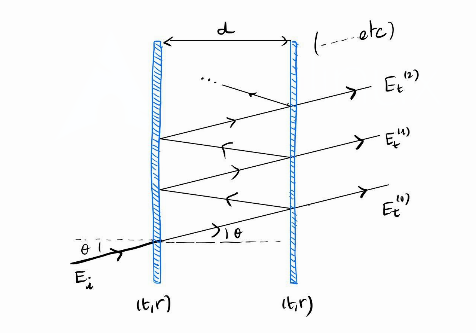
\includegraphics[width=0.8\textwidth]{diagrama.png}
	
	\label{fig:}
\end{figure}
\vspace{0cm}
{\itshape\Large Fenómeno de Interferencia producido por dos láminas semirreflectantes sobre la que incide un haz monocromático \par}
\vfill
{\Large Autores: \par}
{\Large Alberca Berbel, Fernando \par
Gómez Gómez, José Luis \par
Martín Romero, Álvaro}
\vfill
{\Large  \today \par}
\end{titlepage} 


\end{document}
